% Options for packages loaded elsewhere
\PassOptionsToPackage{unicode}{hyperref}
\PassOptionsToPackage{hyphens}{url}
%
\documentclass[
]{article}
\usepackage{amsmath,amssymb}
\usepackage{iftex}
\ifPDFTeX
  \usepackage[T1]{fontenc}
  \usepackage[utf8]{inputenc}
  \usepackage{textcomp} % provide euro and other symbols
\else % if luatex or xetex
  \usepackage{unicode-math} % this also loads fontspec
  \defaultfontfeatures{Scale=MatchLowercase}
  \defaultfontfeatures[\rmfamily]{Ligatures=TeX,Scale=1}
\fi
\usepackage{lmodern}
\ifPDFTeX\else
  % xetex/luatex font selection
\fi
% Use upquote if available, for straight quotes in verbatim environments
\IfFileExists{upquote.sty}{\usepackage{upquote}}{}
\IfFileExists{microtype.sty}{% use microtype if available
  \usepackage[]{microtype}
  \UseMicrotypeSet[protrusion]{basicmath} % disable protrusion for tt fonts
}{}
\makeatletter
\@ifundefined{KOMAClassName}{% if non-KOMA class
  \IfFileExists{parskip.sty}{%
    \usepackage{parskip}
  }{% else
    \setlength{\parindent}{0pt}
    \setlength{\parskip}{6pt plus 2pt minus 1pt}}
}{% if KOMA class
  \KOMAoptions{parskip=half}}
\makeatother
\usepackage{xcolor}
\usepackage[margin=1in]{geometry}
\usepackage{color}
\usepackage{fancyvrb}
\newcommand{\VerbBar}{|}
\newcommand{\VERB}{\Verb[commandchars=\\\{\}]}
\DefineVerbatimEnvironment{Highlighting}{Verbatim}{commandchars=\\\{\}}
% Add ',fontsize=\small' for more characters per line
\usepackage{framed}
\definecolor{shadecolor}{RGB}{248,248,248}
\newenvironment{Shaded}{\begin{snugshade}}{\end{snugshade}}
\newcommand{\AlertTok}[1]{\textcolor[rgb]{0.94,0.16,0.16}{#1}}
\newcommand{\AnnotationTok}[1]{\textcolor[rgb]{0.56,0.35,0.01}{\textbf{\textit{#1}}}}
\newcommand{\AttributeTok}[1]{\textcolor[rgb]{0.13,0.29,0.53}{#1}}
\newcommand{\BaseNTok}[1]{\textcolor[rgb]{0.00,0.00,0.81}{#1}}
\newcommand{\BuiltInTok}[1]{#1}
\newcommand{\CharTok}[1]{\textcolor[rgb]{0.31,0.60,0.02}{#1}}
\newcommand{\CommentTok}[1]{\textcolor[rgb]{0.56,0.35,0.01}{\textit{#1}}}
\newcommand{\CommentVarTok}[1]{\textcolor[rgb]{0.56,0.35,0.01}{\textbf{\textit{#1}}}}
\newcommand{\ConstantTok}[1]{\textcolor[rgb]{0.56,0.35,0.01}{#1}}
\newcommand{\ControlFlowTok}[1]{\textcolor[rgb]{0.13,0.29,0.53}{\textbf{#1}}}
\newcommand{\DataTypeTok}[1]{\textcolor[rgb]{0.13,0.29,0.53}{#1}}
\newcommand{\DecValTok}[1]{\textcolor[rgb]{0.00,0.00,0.81}{#1}}
\newcommand{\DocumentationTok}[1]{\textcolor[rgb]{0.56,0.35,0.01}{\textbf{\textit{#1}}}}
\newcommand{\ErrorTok}[1]{\textcolor[rgb]{0.64,0.00,0.00}{\textbf{#1}}}
\newcommand{\ExtensionTok}[1]{#1}
\newcommand{\FloatTok}[1]{\textcolor[rgb]{0.00,0.00,0.81}{#1}}
\newcommand{\FunctionTok}[1]{\textcolor[rgb]{0.13,0.29,0.53}{\textbf{#1}}}
\newcommand{\ImportTok}[1]{#1}
\newcommand{\InformationTok}[1]{\textcolor[rgb]{0.56,0.35,0.01}{\textbf{\textit{#1}}}}
\newcommand{\KeywordTok}[1]{\textcolor[rgb]{0.13,0.29,0.53}{\textbf{#1}}}
\newcommand{\NormalTok}[1]{#1}
\newcommand{\OperatorTok}[1]{\textcolor[rgb]{0.81,0.36,0.00}{\textbf{#1}}}
\newcommand{\OtherTok}[1]{\textcolor[rgb]{0.56,0.35,0.01}{#1}}
\newcommand{\PreprocessorTok}[1]{\textcolor[rgb]{0.56,0.35,0.01}{\textit{#1}}}
\newcommand{\RegionMarkerTok}[1]{#1}
\newcommand{\SpecialCharTok}[1]{\textcolor[rgb]{0.81,0.36,0.00}{\textbf{#1}}}
\newcommand{\SpecialStringTok}[1]{\textcolor[rgb]{0.31,0.60,0.02}{#1}}
\newcommand{\StringTok}[1]{\textcolor[rgb]{0.31,0.60,0.02}{#1}}
\newcommand{\VariableTok}[1]{\textcolor[rgb]{0.00,0.00,0.00}{#1}}
\newcommand{\VerbatimStringTok}[1]{\textcolor[rgb]{0.31,0.60,0.02}{#1}}
\newcommand{\WarningTok}[1]{\textcolor[rgb]{0.56,0.35,0.01}{\textbf{\textit{#1}}}}
\usepackage{graphicx}
\makeatletter
\def\maxwidth{\ifdim\Gin@nat@width>\linewidth\linewidth\else\Gin@nat@width\fi}
\def\maxheight{\ifdim\Gin@nat@height>\textheight\textheight\else\Gin@nat@height\fi}
\makeatother
% Scale images if necessary, so that they will not overflow the page
% margins by default, and it is still possible to overwrite the defaults
% using explicit options in \includegraphics[width, height, ...]{}
\setkeys{Gin}{width=\maxwidth,height=\maxheight,keepaspectratio}
% Set default figure placement to htbp
\makeatletter
\def\fps@figure{htbp}
\makeatother
\setlength{\emergencystretch}{3em} % prevent overfull lines
\providecommand{\tightlist}{%
  \setlength{\itemsep}{0pt}\setlength{\parskip}{0pt}}
\setcounter{secnumdepth}{-\maxdimen} % remove section numbering
\usepackage{hyperref}
\hypersetup{colorlinks=true, linkcolor=red, urlcolor=blue}
\ifLuaTeX
  \usepackage{selnolig}  % disable illegal ligatures
\fi
\IfFileExists{bookmark.sty}{\usepackage{bookmark}}{\usepackage{hyperref}}
\IfFileExists{xurl.sty}{\usepackage{xurl}}{} % add URL line breaks if available
\urlstyle{same}
\hypersetup{
  pdftitle={(Fast) Introduction to R},
  pdfauthor={Joana Cima},
  hidelinks,
  pdfcreator={LaTeX via pandoc}}

\title{(Fast) Introduction to R}
\usepackage{etoolbox}
\makeatletter
\providecommand{\subtitle}[1]{% add subtitle to \maketitle
  \apptocmd{\@title}{\par {\large #1 \par}}{}{}
}
\makeatother
\subtitle{Jump into a notebook}
\author{Joana Cima}
\date{11 outubro 2023}

\begin{document}
\maketitle

\hypertarget{my-beamer}{%
\section{My beamer}\label{my-beamer}}

\begin{quote}
BlaBlaBla
\end{quote}

\hypertarget{outline}{%
\section{Outline}\label{outline}}

\begin{enumerate}
\def\labelenumi{\arabic{enumi}.}
\tightlist
\item
  Motivation
\item
  Data
\item
  Conceptual discussion
\end{enumerate}

\hypertarget{import-data-from-an-excel-file}{%
\section{3. Import data (from an excel
file)}\label{import-data-from-an-excel-file}}

\hypertarget{load-your-data-using-point-and-click}{%
\subsection{Load your data using point and
click}\label{load-your-data-using-point-and-click}}

\begin{figure}
\centering
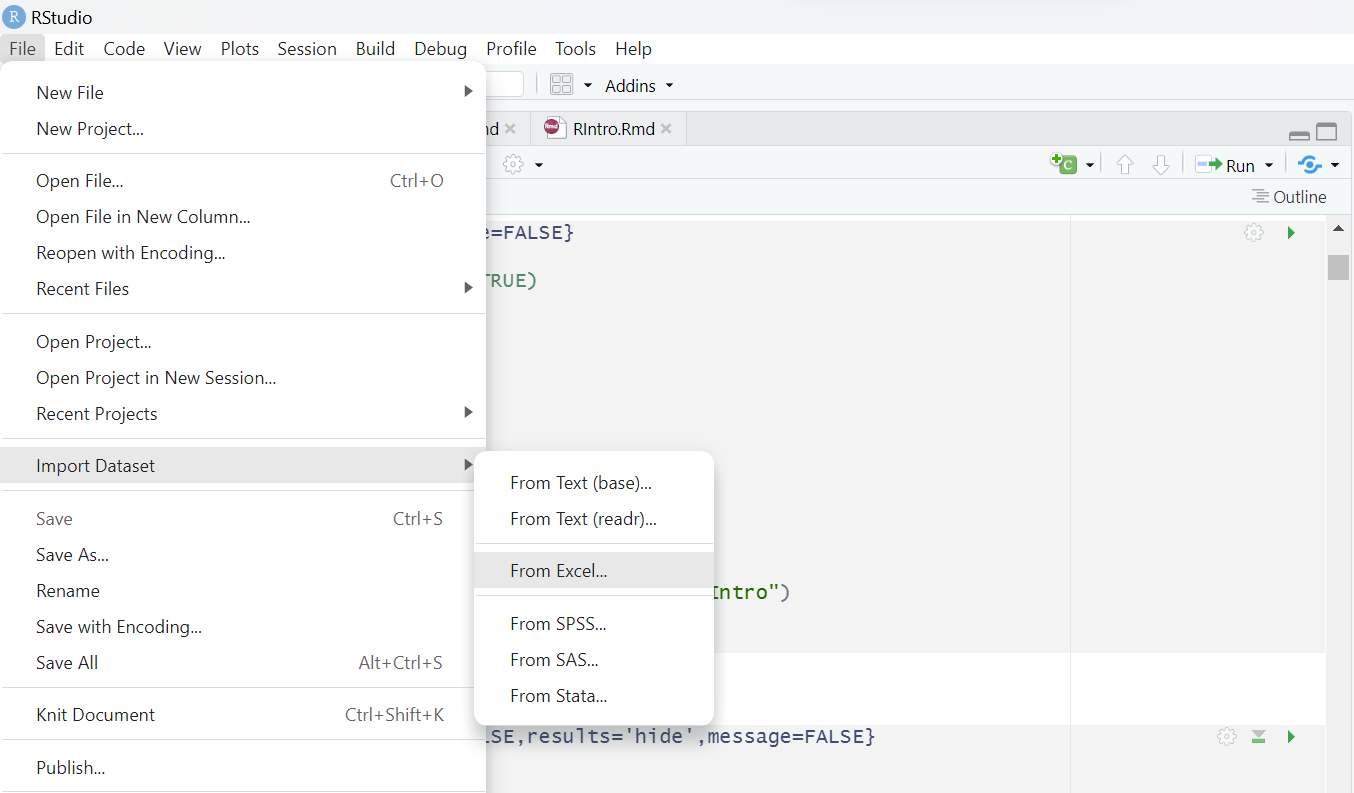
\includegraphics[width=0.31\textwidth,height=\textheight]{importdataset.png}
\caption{Point and click}
\end{figure}

which corresponds to the following code

\begin{Shaded}
\begin{Highlighting}[]
\NormalTok{nlswork }\OtherTok{\textless{}{-}} \FunctionTok{as.data.frame}\NormalTok{(}\FunctionTok{read\_excel}\NormalTok{(}\StringTok{"nlswork.xlsx"}\NormalTok{))}
\CommentTok{\# nlswork \textless{}{-} read\_dta("nlswork.dta") \# in case you have a Stata data source}
\end{Highlighting}
\end{Shaded}

\hypertarget{data-manipulation-check-the-pipe-operator}{%
\section{4. Data manipulation -- check the pipe operator,
\%\textgreater\%}\label{data-manipulation-check-the-pipe-operator}}

\hypertarget{select-a-subset-of-variables}{%
\subsection{4.1. Select a subset of
variables}\label{select-a-subset-of-variables}}

\begin{Shaded}
\begin{Highlighting}[]
\NormalTok{nlswork\_s}\OtherTok{\textless{}{-}}\NormalTok{ nlswork }\SpecialCharTok{\%\textgreater{}\%} 
  \FunctionTok{select}\NormalTok{(idcode, ln\_wage) }
\end{Highlighting}
\end{Shaded}

\hypertarget{rename-variables}{%
\subsection{4.2. Rename variables}\label{rename-variables}}

\begin{Shaded}
\begin{Highlighting}[]
\NormalTok{nlswork\_r }\OtherTok{\textless{}{-}}\NormalTok{ nlswork }\SpecialCharTok{\%\textgreater{}\%} 
  \FunctionTok{rename}\NormalTok{(}\AttributeTok{cae =}\NormalTok{ ind\_code)}
\end{Highlighting}
\end{Shaded}

\hypertarget{filter-a-subset-of-observations}{%
\subsection{4.3. Filter a subset of
observations}\label{filter-a-subset-of-observations}}

\begin{Shaded}
\begin{Highlighting}[]
\NormalTok{nlswork\_f}\OtherTok{\textless{}{-}}\NormalTok{ nlswork }\SpecialCharTok{\%\textgreater{}\%} 
  \FunctionTok{filter}\NormalTok{(age }\SpecialCharTok{\textgreater{}} \DecValTok{40}\NormalTok{) }
\end{Highlighting}
\end{Shaded}

\hypertarget{mutate-create-variables}{%
\subsection{4.4. Mutate: create
variables}\label{mutate-create-variables}}

\begin{Shaded}
\begin{Highlighting}[]
\NormalTok{ nlswork\_m }\OtherTok{\textless{}{-}}\NormalTok{ nlswork }\SpecialCharTok{\%\textgreater{}\%} 
  \FunctionTok{mutate}\NormalTok{(}\AttributeTok{ln\_asd=}\FunctionTok{log}\NormalTok{(age))}
\end{Highlighting}
\end{Shaded}

\hypertarget{manipulate-the-data-in-a-single-sequence}{%
\subsection{4.5. Manipulate the data in a single
sequence}\label{manipulate-the-data-in-a-single-sequence}}

\begin{Shaded}
\begin{Highlighting}[]
\NormalTok{nlswork1}\OtherTok{\textless{}{-}}\NormalTok{ nlswork }\SpecialCharTok{\%\textgreater{}\%} 
  \FunctionTok{rename}\NormalTok{(}\AttributeTok{cae =}\NormalTok{ ind\_code) }\SpecialCharTok{\%\textgreater{}\%}
  \FunctionTok{select}\NormalTok{(idcode, ln\_wage, age) }\SpecialCharTok{\%\textgreater{}\%} 
  \FunctionTok{filter}\NormalTok{(age }\SpecialCharTok{\textgreater{}} \DecValTok{40}\NormalTok{) }\SpecialCharTok{\%\textgreater{}\%}
  \FunctionTok{mutate}\NormalTok{(}\AttributeTok{age2=}\NormalTok{age}\SpecialCharTok{\^{}}\DecValTok{2}\NormalTok{)}
\end{Highlighting}
\end{Shaded}

\hypertarget{visualize-missing-information}{%
\section{5. Visualize missing
information:}\label{visualize-missing-information}}

\begin{Shaded}
\begin{Highlighting}[]
\FunctionTok{vis\_miss}\NormalTok{(nlswork)}
\end{Highlighting}
\end{Shaded}

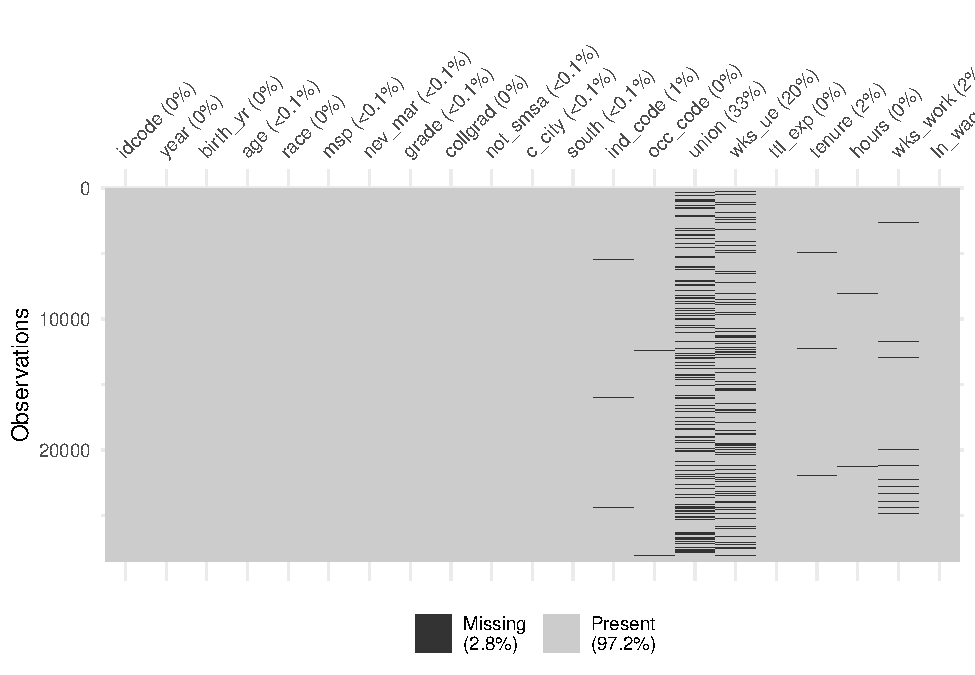
\includegraphics{RIntro_files/figure-latex/unnamed-chunk-7-1.pdf}

\begin{Shaded}
\begin{Highlighting}[]
\FunctionTok{gg\_miss\_var}\NormalTok{(nlswork) }\SpecialCharTok{+} \FunctionTok{labs}\NormalTok{(}\AttributeTok{y =} \StringTok{"Total missing values for each variable"}\NormalTok{)}
\end{Highlighting}
\end{Shaded}

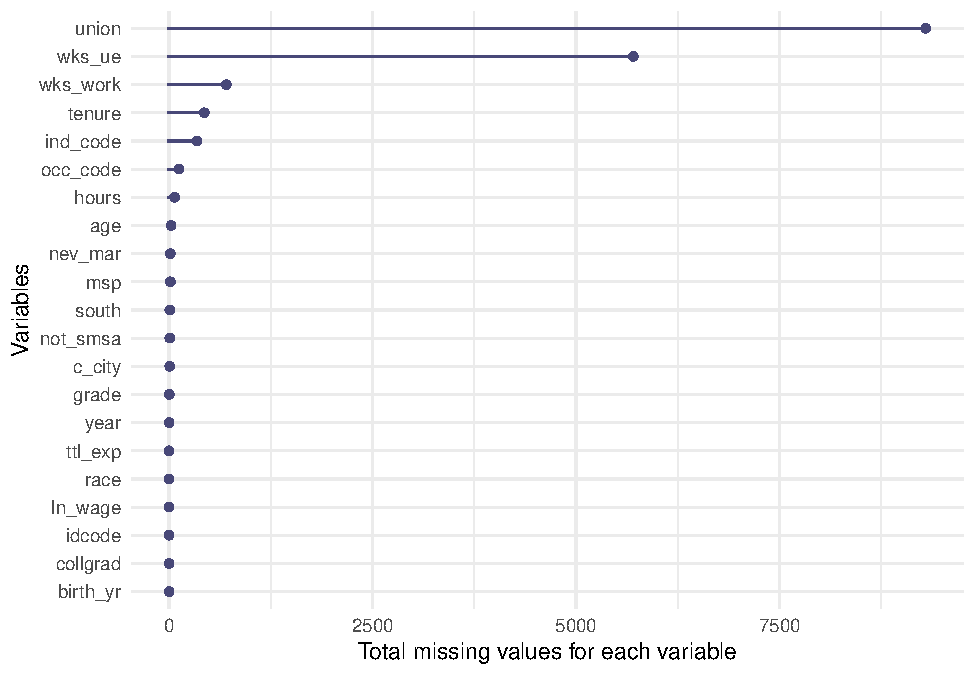
\includegraphics{RIntro_files/figure-latex/unnamed-chunk-8-1.pdf}

\begin{Shaded}
\begin{Highlighting}[]
\FunctionTok{gg\_miss\_upset}\NormalTok{(nlswork)}
\end{Highlighting}
\end{Shaded}

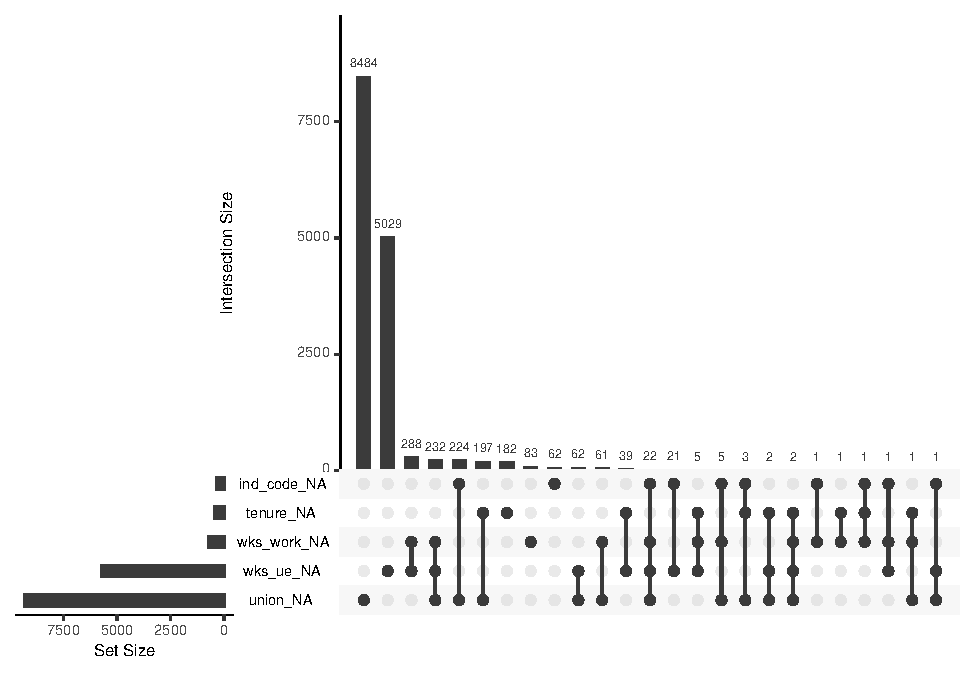
\includegraphics{RIntro_files/figure-latex/unnamed-chunk-8-2.pdf}

\begin{Shaded}
\begin{Highlighting}[]
\FunctionTok{n\_var\_miss}\NormalTok{(nlswork)}
\end{Highlighting}
\end{Shaded}

\begin{verbatim}
## [1] 14
\end{verbatim}

\begin{Shaded}
\begin{Highlighting}[]
\FunctionTok{ggplot}\NormalTok{(nlswork,}\FunctionTok{aes}\NormalTok{(}\AttributeTok{x=}\NormalTok{age,}\AttributeTok{y=}\NormalTok{ln\_wage))}\SpecialCharTok{+}
  \FunctionTok{geom\_point}\NormalTok{()}
\end{Highlighting}
\end{Shaded}

\begin{verbatim}
## Warning: Removed 24 rows containing missing values (`geom_point()`).
\end{verbatim}

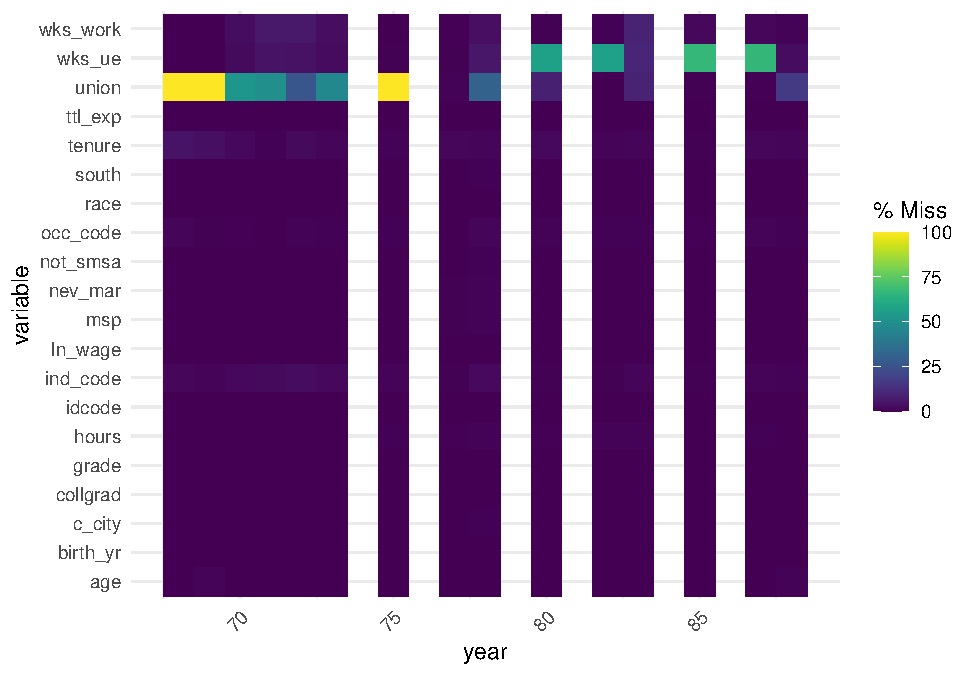
\includegraphics{RIntro_files/figure-latex/unnamed-chunk-9-1.pdf}

\begin{Shaded}
\begin{Highlighting}[]
\FunctionTok{ggplot}\NormalTok{(nlswork,}\FunctionTok{aes}\NormalTok{(}\AttributeTok{x=}\NormalTok{age,}\AttributeTok{y=}\NormalTok{ln\_wage))}\SpecialCharTok{+}
  \FunctionTok{geom\_miss\_point}\NormalTok{()}
\end{Highlighting}
\end{Shaded}

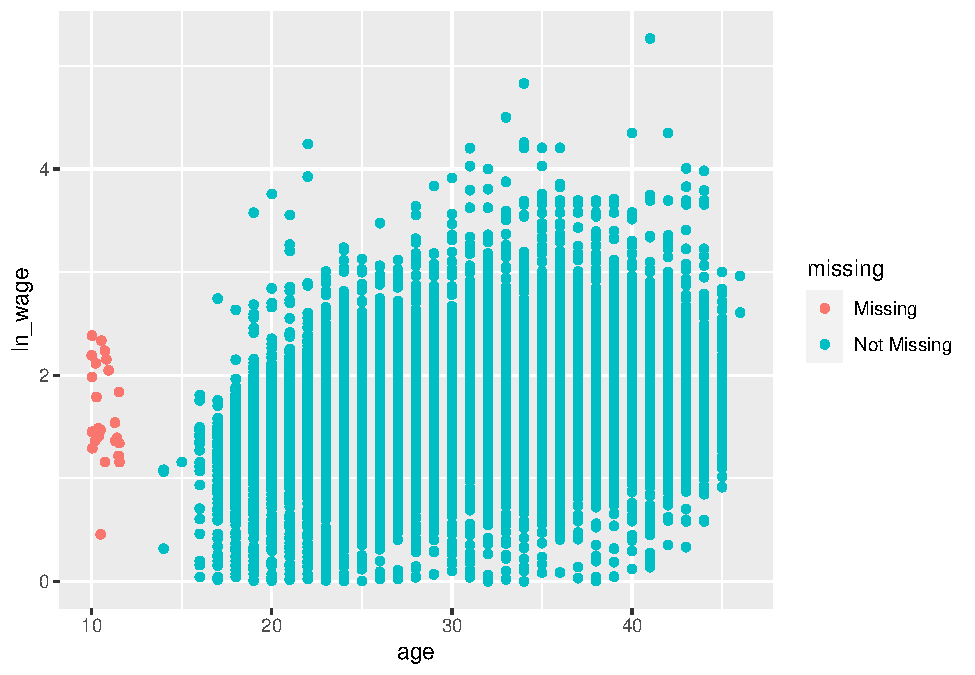
\includegraphics{RIntro_files/figure-latex/unnamed-chunk-9-2.pdf}

\begin{Shaded}
\begin{Highlighting}[]
\FunctionTok{ggplot}\NormalTok{(nlswork,}\FunctionTok{aes}\NormalTok{(}\AttributeTok{x=}\NormalTok{age,}\AttributeTok{y=}\NormalTok{ln\_wage))}\SpecialCharTok{+}
  \FunctionTok{geom\_miss\_point}\NormalTok{() }\SpecialCharTok{+}
  \FunctionTok{facet\_wrap}\NormalTok{(}\SpecialCharTok{\textasciitilde{}}\NormalTok{race)}
\end{Highlighting}
\end{Shaded}

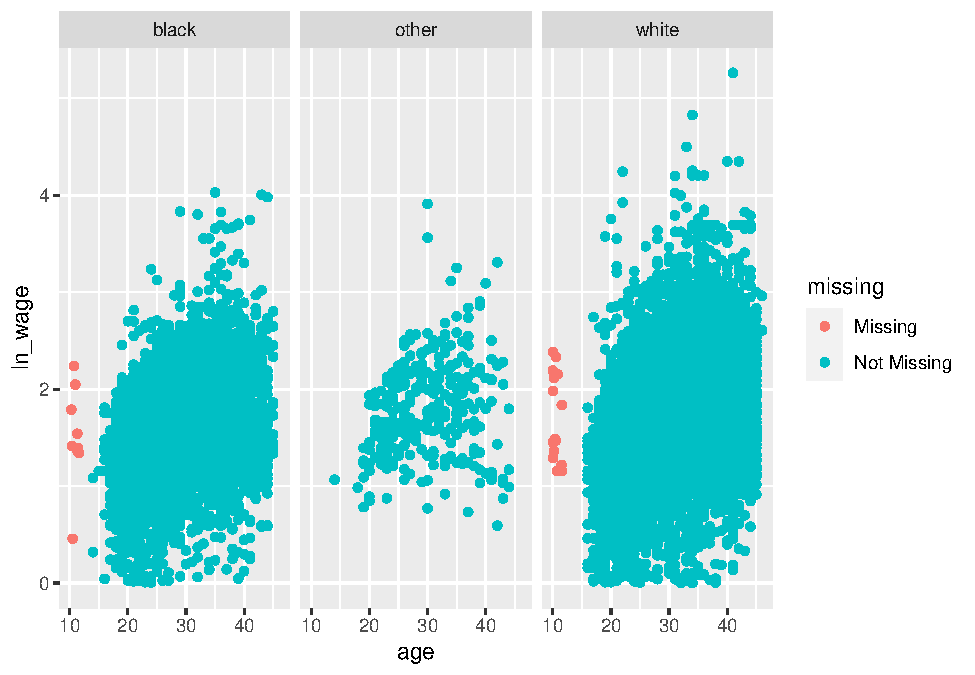
\includegraphics{RIntro_files/figure-latex/unnamed-chunk-9-3.pdf}

\begin{Shaded}
\begin{Highlighting}[]
\FunctionTok{gg\_miss\_fct}\NormalTok{(}\AttributeTok{x =}\NormalTok{ nlswork,}\AttributeTok{fct =}\NormalTok{ year)}
\end{Highlighting}
\end{Shaded}

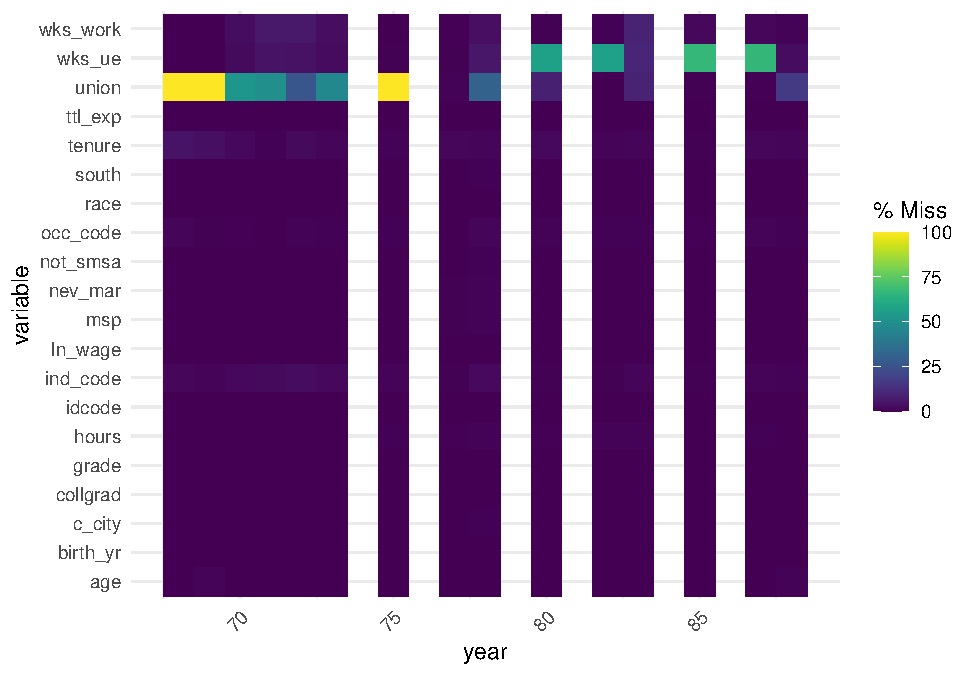
\includegraphics{RIntro_files/figure-latex/unnamed-chunk-9-4.pdf}

\hypertarget{alternative}{%
\subsubsection{Alternative}\label{alternative}}

\begin{Shaded}
\begin{Highlighting}[]
\FunctionTok{vis\_dat}\NormalTok{(nlswork)}
\end{Highlighting}
\end{Shaded}

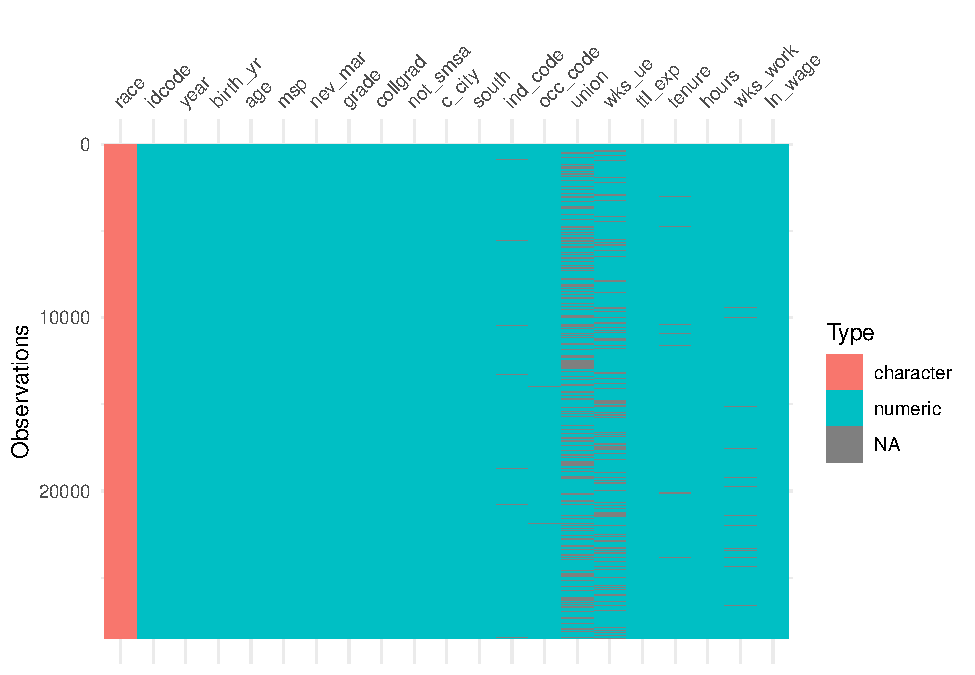
\includegraphics{RIntro_files/figure-latex/unnamed-chunk-10-1.pdf}

\hypertarget{handling-missing-data}{%
\section{6. Handling Missing Data}\label{handling-missing-data}}

Handling missing data is a crucial step in the exploratory data
analysis. Depending on the nature and mechanism of the missingness, we
might decide to impute missing values or to exclude the observations
with missing data.

\hypertarget{filling-missing-data}{%
\subsection{6.1 Filling Missing Data}\label{filling-missing-data}}

In some situations, we may opt to fill in the missing data. For
instance, one common method involves replacing missing values with the
mean of the variable.

\begin{Shaded}
\begin{Highlighting}[]
\CommentTok{\# Filling Missing Data}
\NormalTok{nlswork\_filled }\OtherTok{\textless{}{-}}\NormalTok{ nlswork }\SpecialCharTok{\%\textgreater{}\%}
  \FunctionTok{mutate}\NormalTok{(}\FunctionTok{across}\NormalTok{(}\FunctionTok{c}\NormalTok{(}\StringTok{"union"}\NormalTok{), }\SpecialCharTok{\textasciitilde{}} \FunctionTok{ifelse}\NormalTok{(}\FunctionTok{is.na}\NormalTok{(.), }\FunctionTok{mean}\NormalTok{(., }\AttributeTok{na.rm =} \ConstantTok{TRUE}\NormalTok{), .))) }
\end{Highlighting}
\end{Shaded}

\hypertarget{excluding-rows-with-missing-data}{%
\subsection{6.2 Excluding rows with missing
data}\label{excluding-rows-with-missing-data}}

\begin{Shaded}
\begin{Highlighting}[]
\CommentTok{\# Or excluding rows with missing data}

\NormalTok{nlswork\_no\_na }\OtherTok{\textless{}{-}} \FunctionTok{na.omit}\NormalTok{(nlswork)}
\end{Highlighting}
\end{Shaded}

\hypertarget{descriptive-statistics}{%
\section{7. Descriptive statistics}\label{descriptive-statistics}}

\begin{Shaded}
\begin{Highlighting}[]
\FunctionTok{summary}\NormalTok{(nlswork\_no\_na) }
\end{Highlighting}
\end{Shaded}

\begin{verbatim}
##      idcode          year          birth_yr          age      
##  Min.   :   1   Min.   :70.00   Min.   :41.00   Min.   :16.0  
##  1st Qu.:1280   1st Qu.:73.00   1st Qu.:46.00   1st Qu.:25.0  
##  Median :2594   Median :78.00   Median :48.00   Median :30.0  
##  Mean   :2589   Mean   :79.12   Mean   :48.11   Mean   :30.2  
##  3rd Qu.:3859   3rd Qu.:83.00   3rd Qu.:51.00   3rd Qu.:35.0  
##  Max.   :5159   Max.   :88.00   Max.   :54.00   Max.   :46.0  
##      race                msp            nev_mar           grade      
##  Length:13452       Min.   :0.0000   Min.   :0.0000   Min.   : 0.00  
##  Class :character   1st Qu.:0.0000   1st Qu.:0.0000   1st Qu.:12.00  
##  Mode  :character   Median :1.0000   Median :0.0000   Median :12.00  
##                     Mean   :0.6257   Mean   :0.2081   Mean   :12.68  
##                     3rd Qu.:1.0000   3rd Qu.:0.0000   3rd Qu.:14.00  
##                     Max.   :1.0000   Max.   :1.0000   Max.   :18.00  
##     collgrad         not_smsa         c_city           south       
##  Min.   :0.0000   Min.   :0.000   Min.   :0.0000   Min.   :0.0000  
##  1st Qu.:0.0000   1st Qu.:0.000   1st Qu.:0.0000   1st Qu.:0.0000  
##  Median :0.0000   Median :0.000   Median :0.0000   Median :0.0000  
##  Mean   :0.1887   Mean   :0.284   Mean   :0.3417   Mean   :0.4081  
##  3rd Qu.:0.0000   3rd Qu.:1.000   3rd Qu.:1.0000   3rd Qu.:1.0000  
##  Max.   :1.0000   Max.   :1.000   Max.   :1.0000   Max.   :1.0000  
##     ind_code         occ_code          union            wks_ue      
##  Min.   : 1.000   Min.   : 1.000   Min.   :0.0000   Min.   : 0.000  
##  1st Qu.: 5.000   1st Qu.: 3.000   1st Qu.:0.0000   1st Qu.: 0.000  
##  Median : 7.000   Median : 3.000   Median :0.0000   Median : 0.000  
##  Mean   : 7.842   Mean   : 4.839   Mean   :0.2286   Mean   : 2.112  
##  3rd Qu.:11.000   3rd Qu.: 6.000   3rd Qu.:0.0000   3rd Qu.: 0.000  
##  Max.   :12.000   Max.   :13.000   Max.   :1.0000   Max.   :75.000  
##     ttl_exp           tenure            hours          wks_work     
##  Min.   : 0.000   Min.   : 0.0000   Min.   :  1.0   Min.   :  0.00  
##  1st Qu.: 3.417   1st Qu.: 0.8333   1st Qu.: 35.0   1st Qu.: 43.00  
##  Median : 5.635   Median : 2.0833   Median : 40.0   Median : 52.00  
##  Mean   : 6.773   Mean   : 3.4475   Mean   : 36.2   Mean   : 50.73  
##  3rd Qu.: 9.263   3rd Qu.: 4.5000   3rd Qu.: 40.0   3rd Qu.: 58.00  
##  Max.   :28.885   Max.   :25.9167   Max.   :168.0   Max.   :103.00  
##     ln_wage     
##  Min.   :0.000  
##  1st Qu.:1.397  
##  Median :1.690  
##  Mean   :1.714  
##  3rd Qu.:2.001  
##  Max.   :5.264
\end{verbatim}

\begin{Shaded}
\begin{Highlighting}[]
\FunctionTok{summary}\NormalTok{(nlswork\_no\_na[,}\FunctionTok{c}\NormalTok{(}\StringTok{"grade"}\NormalTok{,}\StringTok{"union"}\NormalTok{,}\StringTok{"ln\_wage"}\NormalTok{)]) }
\end{Highlighting}
\end{Shaded}

\begin{verbatim}
##      grade           union           ln_wage     
##  Min.   : 0.00   Min.   :0.0000   Min.   :0.000  
##  1st Qu.:12.00   1st Qu.:0.0000   1st Qu.:1.397  
##  Median :12.00   Median :0.0000   Median :1.690  
##  Mean   :12.68   Mean   :0.2286   Mean   :1.714  
##  3rd Qu.:14.00   3rd Qu.:0.0000   3rd Qu.:2.001  
##  Max.   :18.00   Max.   :1.0000   Max.   :5.264
\end{verbatim}

\begin{Shaded}
\begin{Highlighting}[]
\FunctionTok{str}\NormalTok{(nlswork\_no\_na) }
\end{Highlighting}
\end{Shaded}

\begin{verbatim}
## 'data.frame':    13452 obs. of  21 variables:
##  $ idcode  : num  1 1 1 1 1 1 2 2 2 2 ...
##  $ year    : num  72 77 80 85 87 88 71 77 78 83 ...
##  $ birth_yr: num  51 51 51 51 51 51 51 51 51 51 ...
##  $ age     : num  20 25 28 33 35 37 19 25 26 31 ...
##  $ race    : chr  "black" "black" "black" "black" ...
##  $ msp     : num  1 0 0 0 0 0 1 1 1 1 ...
##  $ nev_mar : num  0 0 0 0 0 0 0 0 0 0 ...
##  $ grade   : num  12 12 12 12 12 12 12 12 12 12 ...
##  $ collgrad: num  0 0 0 0 0 0 0 0 0 0 ...
##  $ not_smsa: num  0 0 0 0 0 0 0 0 0 0 ...
##  $ c_city  : num  1 1 1 1 0 0 1 1 1 1 ...
##  $ south   : num  0 0 0 0 0 0 0 0 0 0 ...
##  $ ind_code: num  4 12 5 5 5 5 4 4 4 4 ...
##  $ occ_code: num  6 8 6 6 6 6 3 6 6 6 ...
##  $ union   : num  1 0 1 1 1 1 0 1 1 1 ...
##  $ wks_ue  : num  0 0 0 0 0 0 19 0 0 12 ...
##  $ ttl_exp : num  2.26 3.78 5.29 7.16 8.99 ...
##  $ tenure  : num  0.917 1.5 1.833 1.917 3.917 ...
##  $ hours   : num  40 32 45 42 45 48 40 40 40 38 ...
##  $ wks_work: num  51 52 75 97 95 70 13 52 52 37 ...
##  $ ln_wage : num  1.59 1.78 2.55 2.61 2.54 ...
##  - attr(*, "na.action")= 'omit' Named int [1:15082] 1 2 4 5 7 9 14 15 16 19 ...
##   ..- attr(*, "names")= chr [1:15082] "1" "2" "4" "5" ...
\end{verbatim}

\hypertarget{shorter-statistics}{%
\section{Shorter statistics}\label{shorter-statistics}}

\hypertarget{statistic-min-mean-st.-dev.-max}{%
\subsection{Statistic Min Mean St.~Dev.
Max}\label{statistic-min-mean-st.-dev.-max}}

Collage Graduate 0 0.19 0.39 1\\
Experience 0.00 6.77 4.41 28.88 Hours 1 36.20 10.03 168
------------------------------------------

\hypertarget{export-descriptive-statistics-table-to-html-with-2-digits}{%
\subsection{7.1. Export descriptive statistics table to html, with 2
digits}\label{export-descriptive-statistics-table-to-html-with-2-digits}}

\begin{Shaded}
\begin{Highlighting}[]
\NormalTok{nlswork\_no\_na }\SpecialCharTok{\%\textgreater{}\%}
\NormalTok{  dplyr}\SpecialCharTok{::}\FunctionTok{select}\NormalTok{(age, collgrad, ttl\_exp, union, hours) }\SpecialCharTok{\%\textgreater{}\%} 
  \FunctionTok{stargazer}\NormalTok{(}\AttributeTok{title=}\StringTok{"Shorter statistics"}\NormalTok{,}
            \AttributeTok{type=} \StringTok{"text"}\NormalTok{, }\AttributeTok{out =} \StringTok{"Statistics\_output.html"}\NormalTok{,}
            \AttributeTok{digits =} \DecValTok{2}\NormalTok{)}
\end{Highlighting}
\end{Shaded}

\begin{verbatim}
## 
## Shorter statistics
## ==========================================
## Statistic   N    Mean  St. Dev. Min   Max 
## ------------------------------------------
## age       13,452 30.20   6.41    16   46  
## collgrad  13,452 0.19    0.39    0     1  
## ttl_exp   13,452 6.77    4.41   0.00 28.88
## union     13,452 0.23    0.42    0     1  
## hours     13,452 36.20  10.03    1    168 
## ------------------------------------------
\end{verbatim}

\hypertarget{export-descriptive-statistics-table-to-txt-with-3-digits}{%
\subsection{7.2. Export descriptive statistics table to txt, with 3
digits}\label{export-descriptive-statistics-table-to-txt-with-3-digits}}

\begin{Shaded}
\begin{Highlighting}[]
\NormalTok{nlswork\_no\_na }\SpecialCharTok{\%\textgreater{}\%}
\NormalTok{  dplyr}\SpecialCharTok{::}\FunctionTok{select}\NormalTok{(age, collgrad, ttl\_exp, union, hours) }\SpecialCharTok{\%\textgreater{}\%} 
  \FunctionTok{stargazer}\NormalTok{(}\AttributeTok{title=}\StringTok{"Shorter statistics"}\NormalTok{,}
            \AttributeTok{type=} \StringTok{"text"}\NormalTok{, }\AttributeTok{out =} \StringTok{"Statistics\_output.txt"}\NormalTok{,}
            \AttributeTok{digits =} \DecValTok{3}\NormalTok{)}
\end{Highlighting}
\end{Shaded}

\begin{verbatim}
## 
## Shorter statistics
## =============================================
## Statistic   N     Mean  St. Dev.  Min   Max  
## ---------------------------------------------
## age       13,452 30.203  6.414    16     46  
## collgrad  13,452 0.189   0.391     0     1   
## ttl_exp   13,452 6.773   4.409   0.000 28.885
## union     13,452 0.229   0.420     0     1   
## hours     13,452 36.199  10.034    1    168  
## ---------------------------------------------
\end{verbatim}

\hypertarget{transposing-the-descriptive-statistics-table}{%
\subsection{7.3. Transposing the descriptive statistics
table}\label{transposing-the-descriptive-statistics-table}}

\begin{Shaded}
\begin{Highlighting}[]
\NormalTok{nlswork\_no\_na }\SpecialCharTok{\%\textgreater{}\%}
\NormalTok{  dplyr}\SpecialCharTok{::}\FunctionTok{select}\NormalTok{(age, collgrad, ttl\_exp, union, hours) }\SpecialCharTok{\%\textgreater{}\%} 
  \FunctionTok{stargazer}\NormalTok{(}\AttributeTok{title=}\StringTok{"Shorter statistics"}\NormalTok{,}
            \AttributeTok{type=} \StringTok{"text"}\NormalTok{, }\AttributeTok{out =} \StringTok{"Statistics\_output2.txt"}\NormalTok{,}
            \AttributeTok{digits =} \DecValTok{3}\NormalTok{, }\AttributeTok{flip=}\ConstantTok{TRUE}\NormalTok{)}
\end{Highlighting}
\end{Shaded}

\begin{verbatim}
## 
## Shorter statistics
## ===============================================
## Statistic  age   collgrad ttl_exp union  hours 
## -----------------------------------------------
## N         13,452  13,452  13,452  13,452 13,452
## Mean      30.203  0.189    6.773  0.229  36.199
## St. Dev.  6.414   0.391    4.409  0.420  10.034
## Min         16      0      0.000    0      1   
## Max         46      1     28.885    1     168  
## -----------------------------------------------
\end{verbatim}

\hypertarget{export-to-pdf}{%
\subsection{7.4. Export to pdf}\label{export-to-pdf}}

\begin{Shaded}
\begin{Highlighting}[]
\NormalTok{nlswork\_no\_na }\SpecialCharTok{\%\textgreater{}\%}
\NormalTok{  dplyr}\SpecialCharTok{::}\FunctionTok{select}\NormalTok{(age, collgrad, ttl\_exp, union, hours) }\SpecialCharTok{\%\textgreater{}\%} 
  \FunctionTok{stargazer}\NormalTok{(}\AttributeTok{title=}\StringTok{"Shorter statistics"}\NormalTok{,}
            \AttributeTok{type=} \StringTok{"latex"}\NormalTok{,}
            \AttributeTok{digits =} \DecValTok{3}\NormalTok{, }\AttributeTok{flip=}\ConstantTok{TRUE}\NormalTok{)}
\end{Highlighting}
\end{Shaded}

\% Table created by stargazer v.5.2.3 by Marek Hlavac, Social Policy
Institute. E-mail: marek.hlavac at gmail.com \% Date and time: qua, out
11, 2023 - 12:26:27

\begin{table}[!htbp] \centering 
  \caption{Shorter statistics} 
  \label{} 
\begin{tabular}{@{\extracolsep{5pt}}lccccc} 
\\[-1.8ex]\hline 
\hline \\[-1.8ex] 
Statistic & age & collgrad & ttl\_exp & union & hours \\ 
\hline \\[-1.8ex] 
N & 13,452 & 13,452 & 13,452 & 13,452 & 13,452 \\ 
Mean & 30.203 & 0.189 & 6.773 & 0.229 & 36.199 \\ 
St. Dev. & 6.414 & 0.391 & 4.409 & 0.420 & 10.034 \\ 
Min & 16 & 0 & 0.000 & 0 & 1 \\ 
Max & 46 & 1 & 28.885 & 1 & 168 \\ 
\hline \\[-1.8ex] 
\end{tabular} 
\end{table}

\hypertarget{visualisation-to-explore-your-data}{%
\section{8. Visualisation to explore your
data}\label{visualisation-to-explore-your-data}}

\hypertarget{relationships-between-continuous-variables}{%
\subsection{8.1. Relationships Between Continuous
Variables}\label{relationships-between-continuous-variables}}

\begin{verbatim}
## `geom_smooth()` using formula = 'y ~ x'
\end{verbatim}

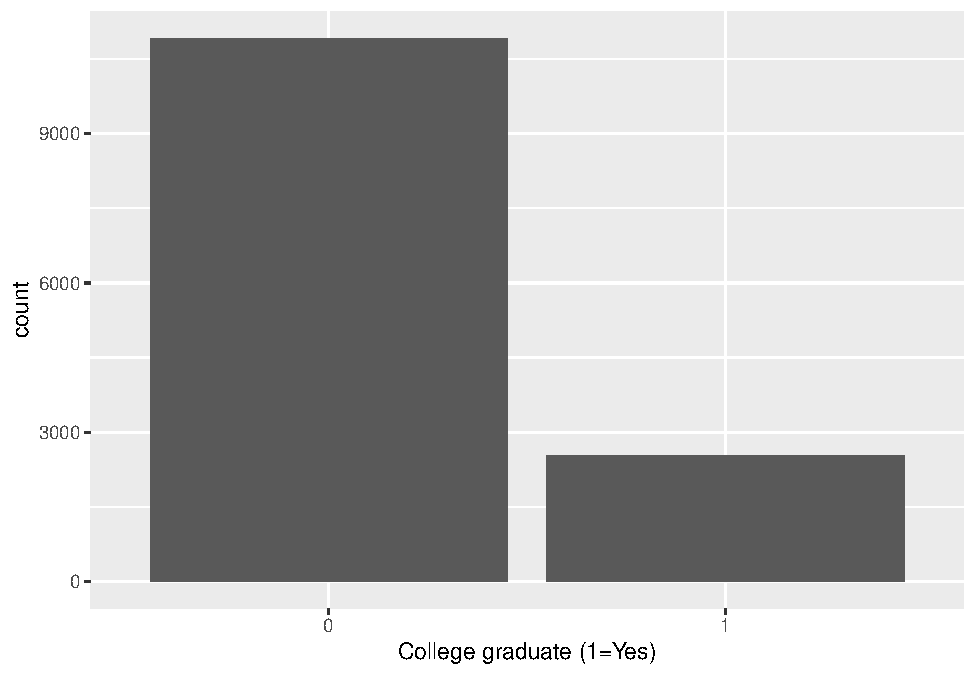
\includegraphics{RIntro_files/figure-latex/unnamed-chunk-19-1.pdf}

\hypertarget{categorical-variable}{%
\subsection{8.2. Categorical variable}\label{categorical-variable}}

\begin{Shaded}
\begin{Highlighting}[]
\FunctionTok{ggplot}\NormalTok{(}\AttributeTok{data =}\NormalTok{ nlswork\_no\_na) }\SpecialCharTok{+}
  \FunctionTok{geom\_bar}\NormalTok{(}\AttributeTok{mapping=}\FunctionTok{aes}\NormalTok{(}\AttributeTok{x=}\FunctionTok{as.factor}\NormalTok{(collgrad))) }\SpecialCharTok{+}
  \FunctionTok{xlab}\NormalTok{(}\StringTok{"College graduate (1=Yes)"}\NormalTok{)}
\end{Highlighting}
\end{Shaded}

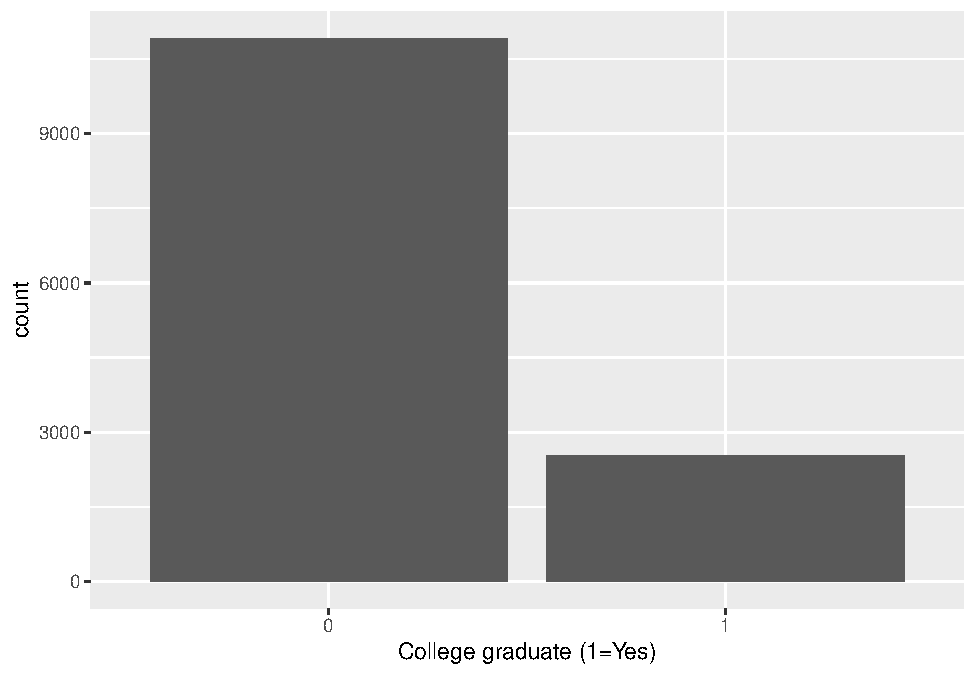
\includegraphics{RIntro_files/figure-latex/unnamed-chunk-20-1.pdf}

\hypertarget{continuous-variable-distributions}{%
\subsection{8.3. Continuous Variable
Distributions}\label{continuous-variable-distributions}}

\begin{Shaded}
\begin{Highlighting}[]
\FunctionTok{ggplot}\NormalTok{(}\AttributeTok{data =}\NormalTok{ nlswork\_no\_na) }\SpecialCharTok{+}
  \FunctionTok{geom\_histogram}\NormalTok{(}\AttributeTok{mapping =} \FunctionTok{aes}\NormalTok{(}\AttributeTok{x =}\NormalTok{ wks\_work), }\AttributeTok{binwidth =} \FloatTok{0.5}\NormalTok{)}
\end{Highlighting}
\end{Shaded}

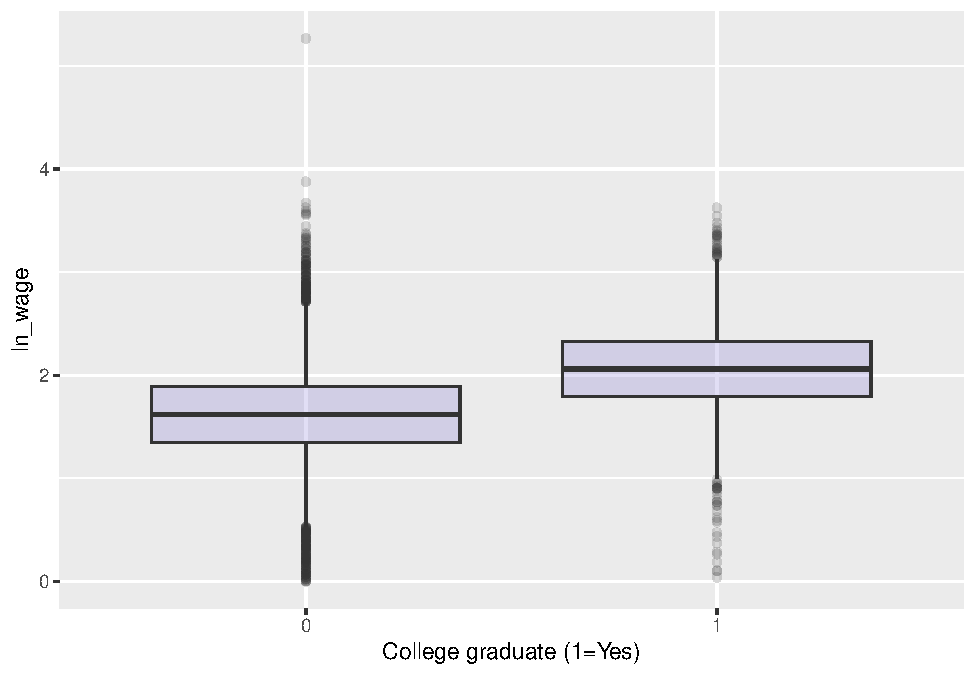
\includegraphics{RIntro_files/figure-latex/unnamed-chunk-21-1.pdf}

\hypertarget{categorical-and-continuous-variables}{%
\subsection{8.4 Categorical and continuous
variables}\label{categorical-and-continuous-variables}}

\begin{Shaded}
\begin{Highlighting}[]
\NormalTok{nlswork\_no\_na }\SpecialCharTok{\%\textgreater{}\%} \FunctionTok{ggplot}\NormalTok{(}\FunctionTok{aes}\NormalTok{(}\AttributeTok{x=}\FunctionTok{as.factor}\NormalTok{(collgrad), }\AttributeTok{y=}\NormalTok{ln\_wage)) }\SpecialCharTok{+}
  \FunctionTok{geom\_boxplot}\NormalTok{(}\AttributeTok{fill=}\StringTok{"slateblue"}\NormalTok{, }\AttributeTok{alpha=}\FloatTok{0.2}\NormalTok{) }\SpecialCharTok{+} 
  \FunctionTok{xlab}\NormalTok{(}\StringTok{"College graduate (1=Yes)"}\NormalTok{)}
\end{Highlighting}
\end{Shaded}

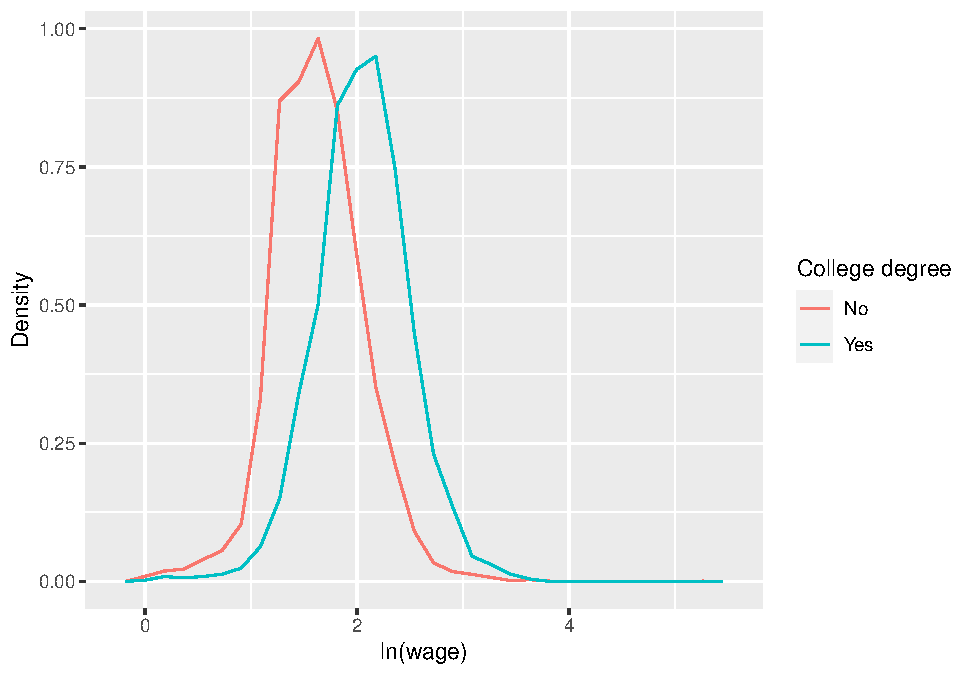
\includegraphics{RIntro_files/figure-latex/unnamed-chunk-22-1.pdf}

\begin{Shaded}
\begin{Highlighting}[]
\NormalTok{nlswork\_no\_na }\SpecialCharTok{\%\textgreater{}\%} \FunctionTok{ggplot}\NormalTok{(}\AttributeTok{mapping =} \FunctionTok{aes}\NormalTok{(}\AttributeTok{x =}\NormalTok{ ln\_wage, }\AttributeTok{y =}\NormalTok{ ..density..)) }\SpecialCharTok{+}
    \FunctionTok{xlab}\NormalTok{(}\StringTok{"ln(wage)"}\NormalTok{) }\SpecialCharTok{+}
    \FunctionTok{ylab}\NormalTok{(}\StringTok{"Density"}\NormalTok{) }\SpecialCharTok{+}
    \FunctionTok{geom\_freqpoly}\NormalTok{(}\AttributeTok{mapping =} \FunctionTok{aes}\NormalTok{(}\AttributeTok{colour =} \FunctionTok{factor}\NormalTok{(collgrad, }\AttributeTok{labels=}\FunctionTok{c}\NormalTok{(}\StringTok{"No"}\NormalTok{, }\StringTok{"Yes"}\NormalTok{)))) }\SpecialCharTok{+}
  \FunctionTok{labs}\NormalTok{(}\AttributeTok{color =}\StringTok{"College degree"}\NormalTok{)}
\end{Highlighting}
\end{Shaded}

\begin{verbatim}
## `stat_bin()` using `bins = 30`. Pick better value with `binwidth`.
\end{verbatim}

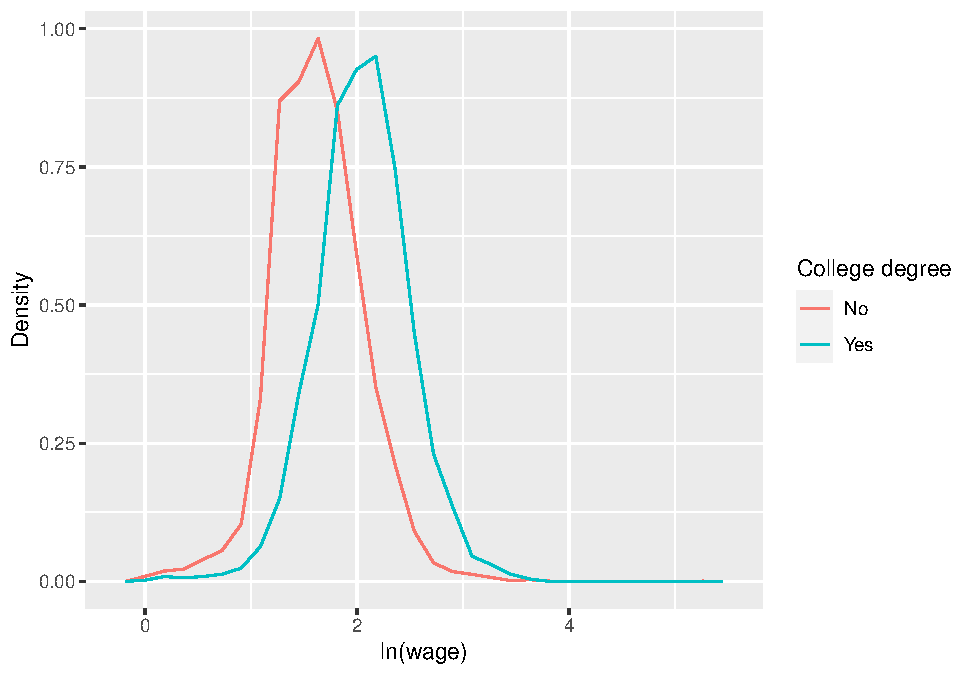
\includegraphics{RIntro_files/figure-latex/unnamed-chunk-23-1.pdf}

\hypertarget{correlation}{%
\section{9. Correlation}\label{correlation}}

\begin{Shaded}
\begin{Highlighting}[]
\FunctionTok{ggpairs}\NormalTok{(nlswork\_no\_na[, }\FunctionTok{c}\NormalTok{(}\StringTok{"age"}\NormalTok{,}\StringTok{"ttl\_exp"}\NormalTok{,}\StringTok{"hours"}\NormalTok{)], }\AttributeTok{title=}\StringTok{"Correlogram with ggpairs()"}\NormalTok{)}
\end{Highlighting}
\end{Shaded}

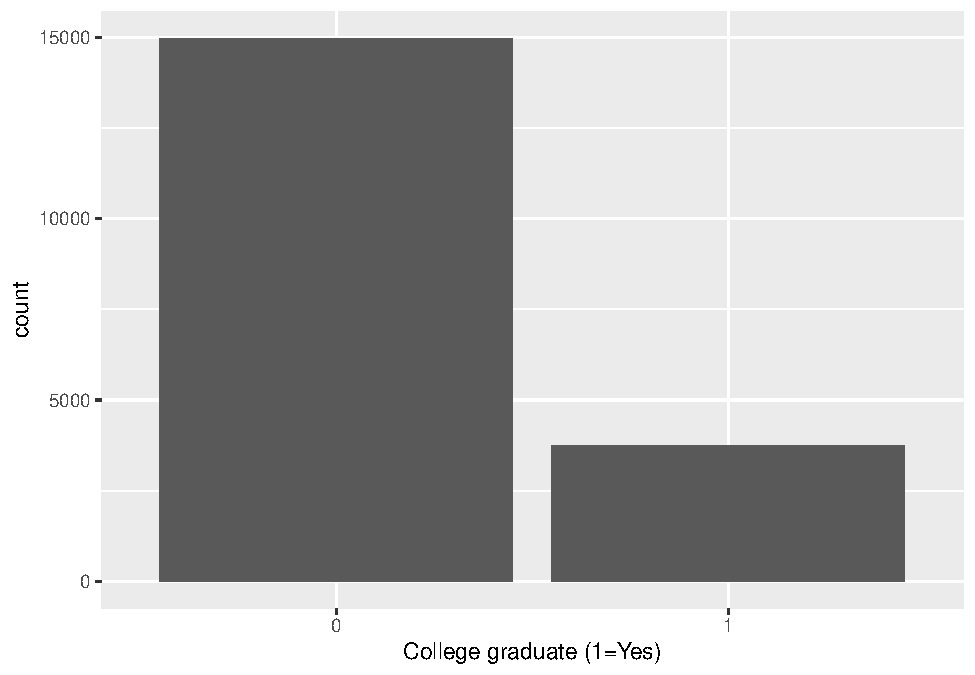
\includegraphics{RIntro_files/figure-latex/unnamed-chunk-24-1.pdf}

\hypertarget{assessment}{%
\section{10. Assessment}\label{assessment}}

\hypertarget{problem-1-data-importing}{%
\subsection{Problem 1: Data Importing}\label{problem-1-data-importing}}

Import the ``card'' dataset.

\begin{Shaded}
\begin{Highlighting}[]
\CommentTok{\#}\RegionMarkerTok{BEGIN}\CommentTok{ SOLUTION}

\CommentTok{\#}\RegionMarkerTok{END}\CommentTok{ SOLUTION}
\end{Highlighting}
\end{Shaded}

\hypertarget{problem-2-visualizing-missing-data}{%
\subsection{Problem 2: Visualizing Missing
Data}\label{problem-2-visualizing-missing-data}}

Graphically show which variables have the most missing values.

\begin{Shaded}
\begin{Highlighting}[]
\CommentTok{\#}\RegionMarkerTok{BEGIN}\CommentTok{ SOLUTION}

\CommentTok{\#}\RegionMarkerTok{END}\CommentTok{ SOLUTION}
\end{Highlighting}
\end{Shaded}

\hypertarget{problem-3-handling-missing-data}{%
\subsection{Problem 3: Handling Missing
Data}\label{problem-3-handling-missing-data}}

Adopt a strategy to handle the missing values.How many observations were
lost?

\begin{Shaded}
\begin{Highlighting}[]
\CommentTok{\#}\RegionMarkerTok{BEGIN}\CommentTok{ SOLUTION}

\CommentTok{\#}\RegionMarkerTok{END}\CommentTok{ SOLUTION}
\end{Highlighting}
\end{Shaded}

\hypertarget{problem-4-descriptive-statistics-after-missing-data-handling}{%
\subsection{Problem 4: Descriptive Statistics after Missing Data
Handling}\label{problem-4-descriptive-statistics-after-missing-data-handling}}

Present statistics of the dataset that has been treated for missing
values.

\begin{Shaded}
\begin{Highlighting}[]
\CommentTok{\#}\RegionMarkerTok{BEGIN}\CommentTok{ SOLUTION}

\CommentTok{\#}\RegionMarkerTok{END}\CommentTok{ SOLUTION}
\end{Highlighting}
\end{Shaded}

\hypertarget{problem-5-relationship-visualization}{%
\subsection{Problem 5: Relationship
Visualization}\label{problem-5-relationship-visualization}}

Graphically show the relationship between age and salary.Does the
relationship between the variables make sense?

\begin{Shaded}
\begin{Highlighting}[]
\CommentTok{\#}\RegionMarkerTok{BEGIN}\CommentTok{ SOLUTION}

\CommentTok{\#}\RegionMarkerTok{END}\CommentTok{ SOLUTION}
\end{Highlighting}
\end{Shaded}

\hypertarget{problem-6-age-distribution}{%
\subsection{Problem 6: Age
Distribution}\label{problem-6-age-distribution}}

Display the distribution of age.

\begin{Shaded}
\begin{Highlighting}[]
\CommentTok{\#}\RegionMarkerTok{BEGIN}\CommentTok{ SOLUTION}

\CommentTok{\#}\RegionMarkerTok{END}\CommentTok{ SOLUTION}
\end{Highlighting}
\end{Shaded}

\hypertarget{problem-7-correlation}{%
\subsection{Problem 7: Correlation}\label{problem-7-correlation}}

What is the correlation value between age and salary?

\begin{Shaded}
\begin{Highlighting}[]
\CommentTok{\#}\RegionMarkerTok{BEGIN}\CommentTok{ SOLUTION}

\CommentTok{\#}\RegionMarkerTok{END}\CommentTok{ SOLUTION}
\end{Highlighting}
\end{Shaded}

\hypertarget{problem-8}{%
\subsection{Problem 8:}\label{problem-8}}

In the nlswork\_no\_na dataset, can you identify any patterns or trends
in the data related to unionized workers and their salaries?

\begin{Shaded}
\begin{Highlighting}[]
\CommentTok{\#}\RegionMarkerTok{BEGIN}\CommentTok{ SOLUTION}

\CommentTok{\#}\RegionMarkerTok{END}\CommentTok{ SOLUTION}
\end{Highlighting}
\end{Shaded}


\end{document}
